\documentclass{beamer}
\usepackage[english]{babel}

\usepackage{lipsum}
\usepackage{style}

% Theme based on https://github.com/elauksap/beamerthemepolimi
\usetheme[bgphoto]{polimi}
\usefonttheme[onlymath]{serif}

% Set custom font (requires to compile with XeLaTeX).
\usepackage{ifxetex}
\ifxetex
    \usepackage{fontspec}
    \setsansfont[Scale=0.95]{Brandon Grotesque}
\fi

\title{\tlap}
\subtitle{%
    A modeling language for
    \texorpdfstring{\linebreak}{}%
    concurrent and distributed systems
}
\author{M. DONADONI \and A. FULGINI \and E. MORASSUTTO}

\begin{document}
    \begin{frame}
        \maketitle
        % If the theme option "nologo" is specified, a custom logo
        % can be added with the following commands:
        %\begin{tikzpicture}[overlay, remember picture]
        %    \node at (current page.north) [anchor=north, inner sep=2cm]
        %    {
        %        
\includegraphics[width=0.3\paperwidth]{logo_centrato_BN_negativo.png}
        %    };
        %\end{tikzpicture}
    \end{frame}

    \begin{frame}{Table of contents}
      \tableofcontents
    \end{frame}

    \section[image=bgphoto_cut]{Section 1}
    % Section page.
    \begin{frame}[plain]{}
        \sectionpage
    \end{frame}

    \begin{frame}{Slide 1}
        \lipsum[1]
    \end{frame}

    \subsection{Subsection 1.1}
    \begin{frame}[plain]{}
        \subsectionpage
    \end{frame}
    \begin{frame}
        This frame has an empty title.
        \vfill
        \begin{itemize}
            \item item 1
            \begin{itemize}
                \item item 1.1
                \item item 1.2
            \end{itemize}
            \item item 2
            \item item 3
        \end{itemize}
    \end{frame}

    \subsection{Subsection 1.2}
    % Slide without numbering.
    \begin{frame}[nonumber]{Slide 1.2 without numbering}
        \lipsum[2]
    \end{frame}

    \section{Section 2}
    \begin{frame}{Slide 2}
        \begin{block}{Block}
            Text.
        \end{block}
        \pause
        \begin{alertblock}{Alert block}
            Alert \alert{text}.
        \end{alertblock}
        \pause
        \begin{exampleblock}{Example block}
            Example \textcolor{greenPolimi}{text}.
        \end{exampleblock}
    \end{frame}

    \begin{frame}[fragile]{A small example}
        \begin{minipage}{\textwidth}
            In this example we show a tiny bit of TLA+ code
            \begin{tla}
                Action == /\ a' = b + c + "string"
                          /\ UNCHANGED <<b,c>>
            \end{tla}
            \begin{tlatex}
                \@x{\@s{65.6} Action \.{\defeq} \.{\land} a \.{'} \.{=} b \.{+} c
                \.{+}\@w{string}}%
                \@x{\@s{101.61} \.{\land} {\UNCHANGED} {\langle} b ,\, c {\rangle}}%
            \end{tlatex}
        \end{minipage}
    \end{frame}

    \section[image=bgphoto_cut]{Introduction}
\begin{frame}[plain]{}
    \sectionpage
\end{frame}

\begin{frame}{\tlap}
    \tlap is a high-level specification language for modeling concurrent and distributed digital systems:
    \begin{itemize}
        \item Algorithms
        \item Programs
        \item Complex computing systems
    \end{itemize}

    \tlap is based on set theory, first-order logic and the Temporal Logic of Actions (TLA); it uses ordinary, basic math.
\end{frame}

\begin{frame}{Leslie Lamport}
    \begin{columns}[onlytextwidth,T]
        \column{\dimexpr\linewidth-30mm-5mm}
        \tlap is developed by Leslie Lamport
        \begin{itemize}
            \item Original author of \LaTeX, first release in 1984
            \item Fundamental contribution to the theory of distributed systems
            \begin{itemize}
                \item Logical Clocks
                \item Byzantine General's problem
                \item Chandy-Lamport distributed snapshot algorithm
                \item Paxos algorithm
                \item many, many other contributions
            \end{itemize}
            \item Turing Award in 2013 (and many other prizes)
        \end{itemize}

        \column{30mm}
        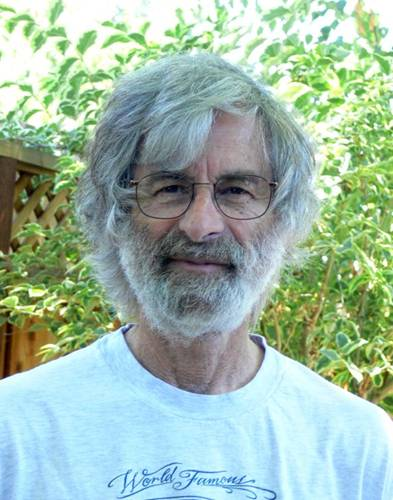
\includegraphics[width=3cm]{images/Leslie_Lamport.jpg}
    \end{columns}
\end{frame}

\begin{frame}{\tlap tooling}
    \setbeamercovered{transparent}
    \begin{description}
        \item<1->[\tlap] specification language
        \item<1->[TLC] model checker and simulator of \tlap specs
        \item<-1>[PlusCal] algorithm language similar to a simple programming language, can be translated to \tlap
        \item<-1>[TLAPS] system for mechanically checking proofs written in \tlap
        \item<-1>[TLATeX] pretty-printer to typeset \tlap specifications in \LaTeX
        \item<1->[Toolbox] IDE for all the \tlap tools
    \end{description}
    \setbeamercovered{invisible}
    \pause
    \vspace{0.5cm}
    \begin{center}
        We will focus on \tlap and TLC and we will use the \tlap Toolbox
    \end{center}
\end{frame}

%TODO: history?

\begin{frame}{Motivations for simple, high-level language}
    Why should we use an high-level language which uses ordinary and simple math instead of some kind of programming language?
    \setbeamercovered{transparent}
    \begin{itemize}[<+->]
        \item It helps us abstract away from implementation details
        \item No special or new syntax, only simple math
        \item Specification of the system is written before the implementation, design errors are found as early as possible
        \item Specification is independent from the language used for implementation
    \end{itemize}
    \setbeamercovered{invisible}
\end{frame}

\begin{frame}{Industrial use of \tlap}
    Who uses \tlap?
    \setbeamercovered{transparent}
    \begin{itemize}
        \item<1> Intel
        \only<1>{
            \begin{itemize}
                \item Used since 2002
                \item Pre-RTL formal verification of cache-coherence protocol
            \end{itemize}
        }
        \item<2> Microsoft
        \only<2>{
            \begin{itemize}
                \item Used since 2004; usage increased in 2015 due to Azure
                \item Found subtle bugs in memory coherence protocol of Xbox 360, Cosmos DB, lock-free data structures
                \item Public specification of the consistency levels of Cosmos DB
            \end{itemize}
        }
        \item<3> OpenComRTOS
        \only<3>{
            \begin{itemize}
                \item New version of \emph{Virtuoso}, the OS of the European Space Agency's \emph{Rosetta} spacecraft
                \item \tlap specification helped to have a cleaner architecture, achieving 10x less code than Virtuoso
            \end{itemize}
        }
        \item<4> Amazon
        \only<4>{
            \begin{itemize}
                \item Used since 2011 for AWS (Amazon Web Services)
                \item As of 2014, used in 10 large complex systems
            \end{itemize}
        }
    \end{itemize}
    \setbeamercovered{invisible}
\end{frame}

\begin{frame}[plain]{Amazon}
    \begin{figure}
        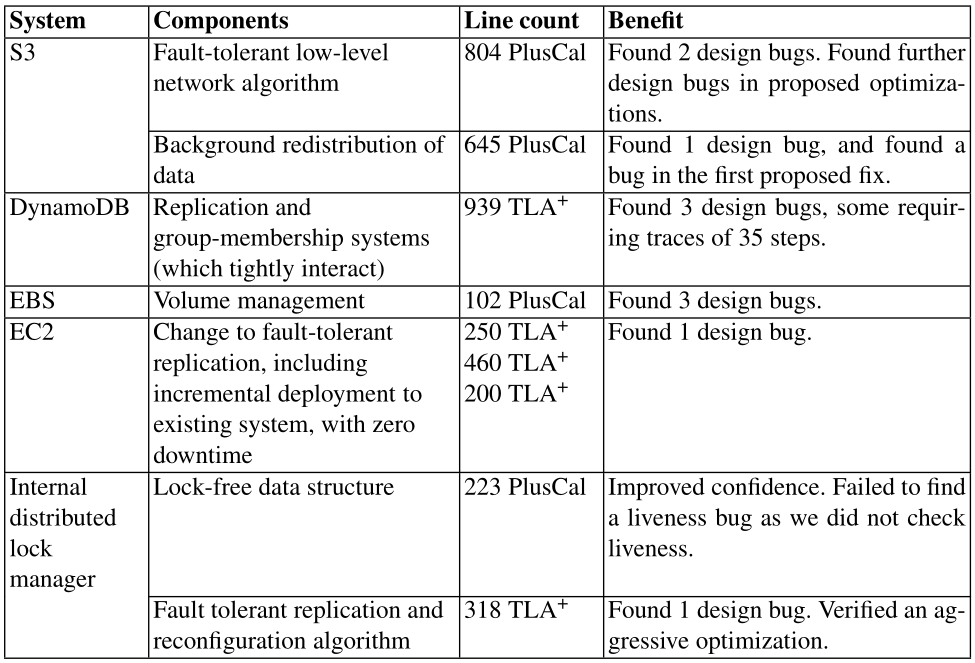
\includegraphics[width=0.9\textwidth]{images/amazon.png}
        \caption{\footnotesize Examples of \tlap usage at Amazon, from \cite{amazon-tla}}
    \end{figure}
\end{frame}

\section[image=bgphoto_cut]{\tlap}
\begin{frame}[plain]{}
    \sectionpage
\end{frame}

\begin{frame}{System description}
    In \tlap, systems are described as \emph{state machines}, using variables.

    \begin{block}{State}
        A \emph{state} of the system is one of the possible assignment of values to the variables.
    \end{block}
    To describe how the system evolves we have to define how the variables change between one state and the next one (transition function).
\end{frame}

\begin{frame}{Variables}
    In \tlap, states are described using \emph{variables}:
    \begin{itemize}
        \item<1-> Numbers or strings
        \item<2-> Sets\\
        \only<2> {
            \begin{center}
                \begin{tabular}{ll}
                    $\left\{ e_1, \dots, e_n \right\}$ & is a generic set\\
                    $\left\{ x \in S : p \right\}$ & is the set of elements of $S$ that satisfy $p$\\
                    $\SUBSET S$ & is the powerset of $S$\\
                \end{tabular}
            \end{center}
        }
        \item<3-> Functions\\
        \only<3> {
            \begin{center}
                \begin{tabularx}{0.9\textwidth}{lX}
                    $f \left[ e \right]$ & is the function application\\
                    $\left[ x \in S \mapsto e \right]$ & is a function such that $f \left[ x \right] = e$ for every $x \in S$\\
                    $\left[ S \rightarrow T \right]$ & is the set of functions from $S$ to $T$\\
                \end{tabularx}
            \end{center}
        }
        \item<4-> Records
        \only<4> {
            \begin{center}
                \begin{tabularx}{0.92\textwidth}{lX}
                    $e.h$ & is the $h$-field of $e$\\
                    $\left[ h_1 \mapsto e_1, \dots, h_n \mapsto e_n \right]$ & is the record whos $h_i$ field is $e_i$\\
                    $\left[ h_1 : S_1, \dots, h_n : S_n \right]$ & is the set of records with $h_i$ field in $S_i$\\
                \end{tabularx}
            \end{center}
        }
        \item<5-> Tuples
        \only<5> {
            \begin{center}
                \begin{tabularx}{0.92\textwidth}{lX}
                    $e \left[ i \right]$ & is the $i$-th component of $e$\\
                    $\left< e_1, \dots, e_n \right>$ & is the $n$-tuple with $e_i$ as the $i$-th component\\
                    $S_1 \times \dots \times S_n$ & is the cartesian product\\
                \end{tabularx}
            \end{center}
        }
    \end{itemize}
\end{frame}

\begin{frame}{Operators}
    These are some of the operators used by \tlap:
    \begin{itemize}
        \item Logical operator such as $\land$, $\lor$, $\neg$, $\implies$, $\equiv$
        \item Quantifiers such as $\forall x \in S : p$ and $\exists x \in S : p$
        \item Set operators $\in$, $\notin$, $\cup$, $\cap$, $\subseteq$, $ \setminus $
        \item Mathematical operators such as $+$, $-$, \dots
    \end{itemize}

\end{frame}

\begin{frame}{State functions and predicates}
    \begin{block}{State function}
    A \emph{state function} is a non-boolean expression built from variables and constants, for example $x^2 + y$.
    \end{block}

    \begin{block}{State predicate}
        A \emph{state predicate} is a boolean expression built from variables and constants, for example $y = 2$.
    \end{block}
\end{frame}

\begin{frame}{Actions}
    How can we describe how the system evolves?
    \pause
    \begin{block}{Action}
        An action represents a relation between a state and the next one and is a boolean-expression formed of variables, constants and \emph{primed variables}. Primed variables refer to the new state.
    \end{block}

    A very simple example of action is $x' = x + 1$.
\end{frame}

\begin{frame}{System specification}
    As we said, in \tlap systems are described as state machines. In particular, we have to define:
    \begin{itemize}
        \item $Init$, a state predicate which characterizes the initial states.
        \item $Next$, which describes the transition function of the system, using actions.
    \end{itemize}
    \pause
    For example, a very simple system with one variable $x$ that can be either incremented or doubled at every step can be defined as:
    \begin{align*}
        Init &\defeq x = 0 \\
        Next &\defeq x' = x+1 \; \lor \; x' = 2 \cdot x\\
    \end{align*}
\end{frame}


    \section[image=bgphoto_cut]{First Modelling Example}
\begin{frame}[plain]{}
    \sectionpage
\end{frame}

\begin{frame}{Simple Clock}
    A $24h$ \textbf{Clock} is a device that keeps time, in our example:
    \setbeamercovered{transparent}
    \begin{itemize}
        \item<1-> It goes from \texttt{00:00} to \texttt{23:59}, ignoring seconds.
        \item<2-> After the minute 59 there is minute 0 and the hour is incremented.
        \item<2-> After the hour reached 23, it goes back to 0.
        \item<3-> The clock should start at 00:00.
    \end{itemize}
    \setbeamercovered{invisible}
\end{frame}

\begin{frame}{Modelling Variables}
    We need to define 2 variables:
    \setbeamercovered{transparent}
    \begin{itemize}[<+->]
        \item \texttt{hr} -- The current hour of the clock
        \item \texttt{min} -- The current minute of the clock\demo
    \end{itemize}
    \setbeamercovered{invisible}
    \onslide<+->
    \vspace{1cm}
    The only valid initial state for the clock is expressed with this predicate:
    \[
        \texttt{hr} = 0 \quad \land \quad \texttt{min} = 0
    \]
    \demo
\end{frame}

\begin{frame}{Modelling Actions}
    \begin{block}{Tick Action}
        \texttt{Tick == AdvanceMin $\land$ AdvanceHr}
    \end{block}
    \pause
    \begin{block}{\texttt{AdvanceMin}}
        The next minute (\texttt{min'}) is the current one (\texttt{min}) plus one. Buf if the minute is already 59, the next is 0.
        \demo
    \end{block}
    \pause
    \begin{block}{\texttt{AdvanceHr}}
        \only<3>{
            \texttt{hr' = hr + 1}\\
            \texttt{\phantom{lol}}\\
            \texttt{\phantom{lol}}\\
            \texttt{\phantom{lol}}\\
            \texttt{\phantom{lol}}\\
        }
        \only<4>{
            \texttt{hr' = IF min < 59}\\
            \texttt{\phantom{hr' = }THEN hr}\\
            \texttt{\phantom{hr' = }ELSE hr + 1}\\
            \texttt{\phantom{lol}}\\
            \texttt{\phantom{lol}}\\
        }
        \only<5->{
            \texttt{hr' = IF min < 59}\\
            \texttt{\phantom{hr' = }THEN hr}\\
            \texttt{\phantom{hr' = }ELSE IF hr < 23}\\
            \texttt{\phantom{hr' = ELSE }THEN hr + 1}\\
            \texttt{\phantom{hr' = ELSE }ELSE 0}
            \demo
        }
    \end{block}
\end{frame}

\begin{frame}{Behavior Specification}
    \begin{block}{Option \#1: Init -- Next}
        The model is defined via the predicate for the initial states (\texttt{Init}), and the only action (\texttt{Tick}).
        \demo
    \end{block}
    \pause
    \begin{block}{Option \#2: TLA formula}
        Specify the behavior using a TLA formula:

        \[
            \texttt{Init} \land \square \texttt{[Tick]}_{\texttt{vars}} \textcolor{gray!60}{\,\land \ldots}
        \]
        \demo

        Note that $\quad\square \texttt{[Tick]}_{\texttt{vars}} \defeq \square ( \texttt{Tick} \lor \texttt{vars'} = \texttt{vars} )$
    \end{block}
\end{frame}

\begin{frame}{Check Temporal Formulae}
    We want to verify some temporal formulae:
    \pause
    \begin{block}{The clock always ticks}
        \[
            \texttt{AlwaysTick == } \square \Diamond \langle \texttt{Tick} \rangle _{\texttt{vars}}
        \]
    \end{block}
    \pause
    \begin{block}{All the possible times are reachable}
        \begin{equation*}
            \begin{gathered}
                \texttt{AllTimes == } \forall h \in (0 \ldots 23), m \in (0 \ldots 59):\\
                \square \Diamond (\texttt{hr = } h\; \land\; \texttt{min = } m)
            \end{gathered}
        \end{equation*}
    \end{block}
    \demo
\end{frame}

\begin{frame}{Fixing the Specification}
    Indeed the specified model is not entirely correct:
    \[
        \texttt{00:00} \rightarrow \texttt{00:00} \rightarrow \texttt{00:00} \rightarrow \texttt{00:00} \rightarrow \cdots
    \]
    It allows an infinite sequence of \emph{stuttering steps}, which is not the correct clock behavior.

    \pause
    We need to add a fairness constraint
    \begin{block}{Fairness constraint}
        \[
            \texttt{LiveClock == Clock } \land \texttt{ WF}_{\texttt{vars}}\texttt{(Tick)}
        \]

        Since \texttt{Tick} is always enabled, it must be \emph{eventually} taken, there must be only a finite number of \emph{stuttering steps} between each \texttt{Tick}.
    \end{block}
    \demo
\end{frame}


    \input{sections/3.twophace.tex}

    \section[image=bgphoto_cut]{\Circle, \emph{Questions?}}
    \begin{frame}{}
        \sectionpage
    \end{frame}
\end{document}
